\documentclass[12pt]{exam}
\usepackage[top=1.5cm,left=2cm,right=2cm]{geometry}
\usepackage{graphicx}
\graphicspath{{../images/}}
\usepackage{listings}
\usepackage{xcolor}
\lstset { %
    language=C++,
    backgroundcolor=\color{black!5}, % set backgroundcolor
    basicstyle=\footnotesize,% basic font setting
}

\usepackage{float}
\usepackage[utf8x]{inputenc}
\usepackage{wasysym}
\usepackage{makecell}
\usepackage{tikz}
\usetikzlibrary{shapes,arrows}
\usetikzlibrary{mindmap}
\pagestyle{headandfoot}
\firstpagefooter{{\bf nota:} Tanto los diagramas de flujo como los programas en c++, deben ser totalmente funcionables y deben ser subidos a un repositorio de Github llamado Examen-Supletorio y su link compartido al classromm Actividad F }{}{}



 
% Define block styles
\tikzstyle{decision} = [diamond, draw, fill=blue!20, text width=3.5em, text badly centered, node distance=1.5cm, inner sep=0pt]
\tikzstyle{block} = [rectangle, draw, fill=blue!20, text centered, rounded corners, minimum
    height=1em, minimum width=0.5cm]
\tikzstyle{line} = [draw, -latex']
\tikzstyle{cloud} = [draw, ellipse,fill=red!10, node distance=2cm,
minimum height=2em]
\tikzstyle{conector}=[circle, scale=0.75, color=white, fill=blue!10]

\tikzstyle{output1} = [signal, signal from=nowhere, signal to=east, minimum width=2cm, minimum height=0.5cm, text centered, draw=black, fill=blue!10]

\tikzstyle{input1} = [signal, signal from=east, signal to=nowhere, minimum width=2cm, minimum height=0.5cm, text centered, draw=black, fill=red!30]






\begin{document}

\thispagestyle{headandfoot}


\begin{minipage}[H]{0.10\linewidth}
  \flushleft
 
\includegraphics[scale=0.12]{images/logoutlvte.png} 
\end{minipage}
\begin{minipage}[H]{0.70\linewidth}
  \begin{center}
    UNIVERSIDAD TÉCNICA LUIS VARGAS TORRES\\  FACULTAD DE INGENIERÍAS\\
    CARRERA DE TECNOLOGÍAS DE LA INFORMACIÓN \\ Examen Supletorio 2021-2S 
  \end{center}
\end{minipage}
\begin{minipage}[H]{0.10\linewidth}
    \flushleft
    
\includegraphics[scale=0.3]{images/logofit}
\end{minipage}

\begin{table}[H]
  \centering
  \begin{tabular}[H]{llll}
    Asignatura: & Fundamentos de Programación & Periodo & 2021-2S\\
              &                     &            & \\     
    Apellidos y nombres: &\rule{7cm}{0.4pt}    &  & \\
              &                     &            & \\
    Fecha: &\rule{5cm}{0.4pt}   & Paralelo: & {\Large B} \\
  \end{tabular}
\end{table}




\begin{questions}

\question[25] Utilizando el diagrama de flujo, diseñar un programa que permita ingresar 4 números y los presente de forma ordenada de mayor a menor. 

  \begin{center}
    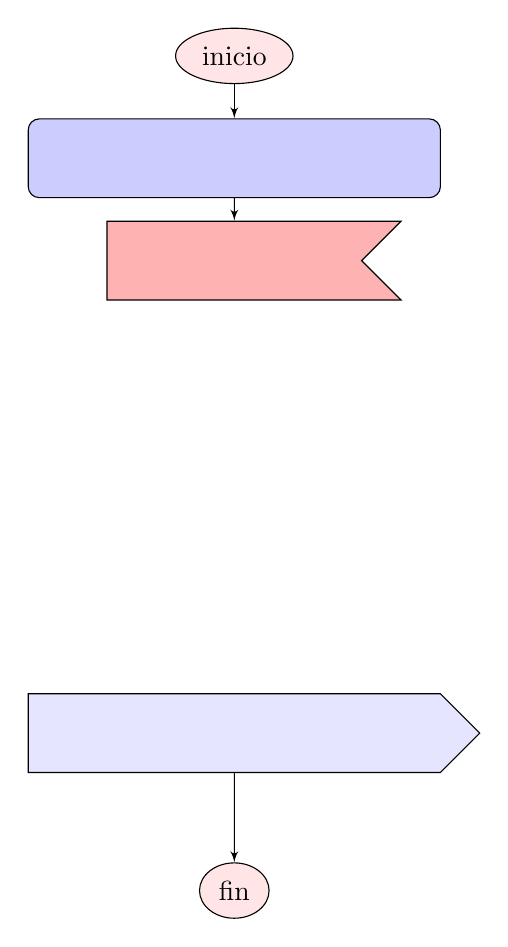
\begin{tikzpicture}[node distance=1cm,auto]
      \node [cloud] (inicio) {inicio};
      \node [block, below  of=inicio,yshift=-0.3cm,text width=5cm,minimum size=1cm]  (declara) {};
      \node [input1, below of=declara,yshift=-0.3cm, text width=3cm,minimum size=1cm] (in1) {};

  
    
   \node [output1, below of=in1, yshift=-5cm,text width=5cm,minimum size=1cm] (out1) {}; 
    
     \node [cloud, below of=out1 ] (fin) {fin};


      \path [line] (inicio) -- (declara);
      \path [line] (declara) --    (in1);
    


     \path [line] (out1) -- (fin);
      
    \end{tikzpicture}
  
  \end{center}

\newpage
\question[25] Utilizando el diagrama de flujo, diseñar un programa  que permita ingresar una hora, minuto, segundo inicial(hi,mi,si) y una hora,minuto, segundo final(hf,mf,sf); el programa calculará las horas, minutos y segundos(ht,mt,st) transcurridos además el programa debe transformar las horas y minutos  a segundos para presentar el resultado solo en segundos. 



  \begin{center}
    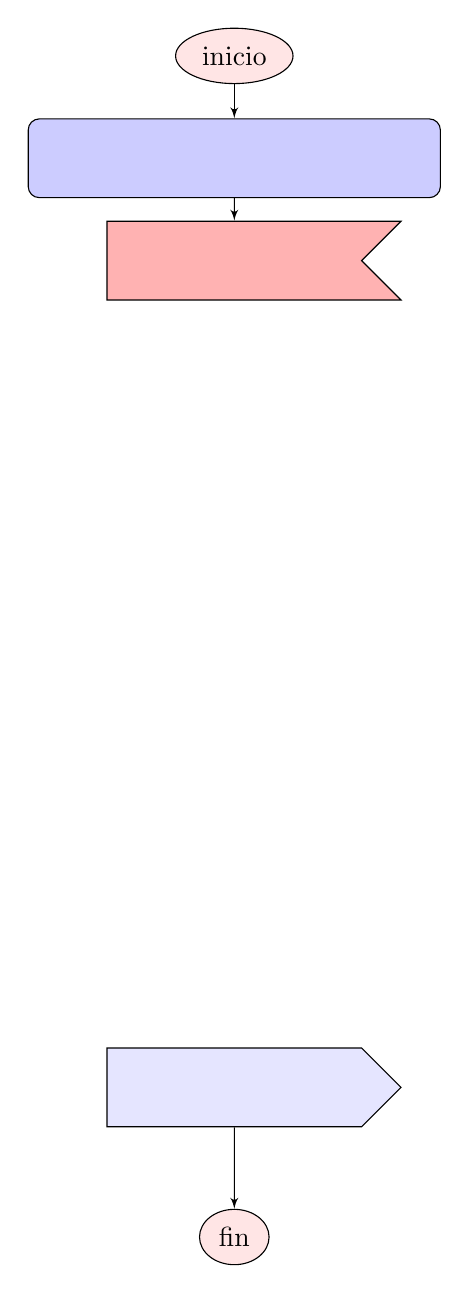
\begin{tikzpicture}[node distance=1cm,auto]
      \node [cloud] (inicio) {inicio};
      \node [block, below  of=inicio,yshift=-0.3cm,text width=5cm,minimum size=1cm]  (declara) {};
      \node [input1, below of=declara,yshift=-0.3cm, text width=3cm,minimum size=1cm] (in1) {};

  
    
   \node [output1, below of=in1, yshift=-9.5cm,text width=3cm,minimum size=1cm] (out1) {}; 
     \node [cloud, below of=out1,yshift=0.1cm ] (fin) {fin};


      \path [line] (inicio) -- (declara);
      \path [line] (declara) --    (in1);
     \path [line] (out1) -- (fin);
      
    \end{tikzpicture}
  
  \end{center}




\newpage
  

\question[25] Crear un programa en c++ que permita ingresar 4 números  y los presente de forma ordenada de mayor a menor. 

  
\begin{lstlisting}
  #include<iostream>
  using namespace std;
  int main()
  {
    //personalizar la variables 
    fload num1,num2,num3,num4;

















    














    

   return 0;
   }
\end{lstlisting}


\newpage
\question[25] Crear un programa en c++  que permita ingresar una hora, minuto, segundo inicial(hi,mi,si) y una hora,minuto, segundo final(hf,mf,sf); el programa calculará las horas, minutos y segundos(ht,mt,st) transcurridos además el programa debe transformar las horas y minutos a segundos para presentar el resultado solo en segundo. 
\vspace{2cm}
\begin{lstlisting}
  #include<iostream>
  using namespace std;
  int main()
  {
    //personalizar la variables ejemplo f_hi
    fload hi,mi,fi, hf,mf,sf,num1,ht,mt,st, totalsegundos;

    















    














    
   cout<<''Total segundos transcurridos : ``<<totalsegundos<<'' Segundos ``<<endl;
   return 0;
   }
\end{lstlisting}









\end{questions}


\end{document}

%%% Local Variables:
%%% mode: latex
%%% TeX-master: t
%%% End:
